\documentclass[letterpaper]{article}

\usepackage [english]{babel}
\usepackage [autostyle, english = american]{csquotes}
\MakeOuterQuote{"}
\usepackage{natbib,alifeconf}  %% The order is important
\usepackage{url}
\usepackage{graphicx}
\graphicspath{ {./pictures/} }

\def\imfig#1#2{\begin{figure}[h] \centering \includegraphics[width=\columnwidth]{#1} \caption{#2} \end{figure}}


% *****************
%  Requirements:
% *****************
%
% - All pages sized consistently at 8.5 x 11 inches (US letter size).
% - PDF length <= 8 pages for full papers, <=2 pages for extended
%    abstracts.
% - Abstract length <= 250 words.
% - No visible crop marks.
% - Images at no greater than 300 dpi, scaled at 100%.
% - Embedded open type fonts only.
% - All layers flattened.
% - No attachments.
% - All desired links active in the files.

% Note that the PDF file must not exceed 5 MB if it is to be indexed
% by Google Scholar. Additional information about Google Scholar
% can be found here:
% http://www.google.com/intl/en/scholar/inclusion.html.


% If your system does not generate letter format documents by default,
% you can use the following workflow:
% latex example
% bibtex example
% latex example ; latex example
% dvips -o example.ps -t letterSize example.dvi
% ps2pdf example.ps example.pdf


% For pdflatex users:
% The alifeconf style file loads the "graphicx" package, and
% this may lead some users of pdflatex to experience problems.
% These can be fixed by editing the alifeconf.sty file to specify:
% \usepackage[pdftex]{graphicx}
%   instead of
% \usepackage{graphicx}.
% The PDF output generated by pdflatex should match the required
% specifications and obviously the dvips and ps2pdf steps become
% unnecessary.


% Note:  Some laser printers have a serious problem printing TeX
% output. The use of ps type I fonts should avoid this problem.


\title{They are Very Smart: Genetic-Algorithm-Based Pathfinding in Games}
\author{Joel Tibbetts and Patrick Nuckolls\\
\mbox{}\\
Grinnell College, Grinnell, IA 50112 \\
} % email of corresponding author

% For several authors from the same institution use the same number to
% refer to one address.
%
% If the names do not fit well on one line use
%         Author 1, Author 2 ... \\ {\Large\bf Author n} ...\\ ...
%
% If the title and author information do not fit in the area
% allocated, place \setlength\titlebox{<new height>} after the
% \documentclass line where <new height> is 2.25in


\def\tavs{\textit{They are Very Smart}}
\begin{document}
\maketitle

\begin{abstract}
\tavs~is a destructible tower defense game that explores the viability of short term evolution of neural nets for pathfinding in an adapting adversarial environment.
\end{abstract}

\section{Introduction}
\tavs~is a real-time tower defense game with evolving enemies; which is to say that the player places down towers and other defenses in real time to fend off waves of enemies attempting to destroy the player's "home base." In typical tower defense games, after killing one group of enemies, another comes which is usually stronger than the previous, due to a pre-ordained set of constraints. \tavs~differs from typical tower defense games in that enemy progression is not determined by the game developer, but rather evolves as a result of a genetic algorithm which controls the enemies' damage, movement speed, health, and navigation.

\begin{figure}[h]
	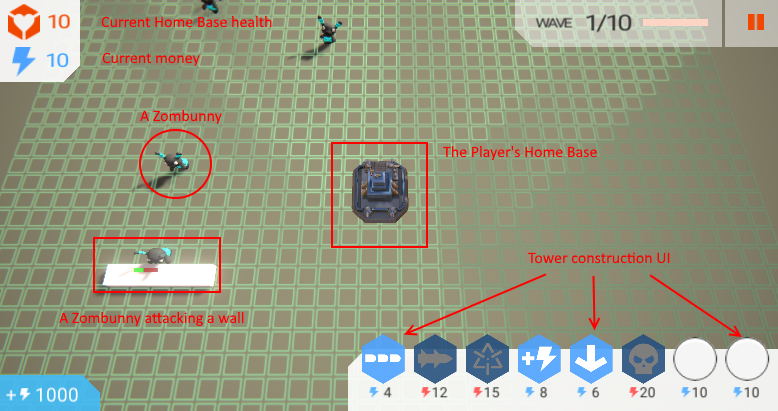
\includegraphics[width=\columnwidth]{InGameLabeled}
	\caption{A screenshot from the game, with various elements labeled}
\end{figure}

In \tavs, player interaction consists of constructing defenses around a central home base. The home base exists in a fixed location in the center of the map, has a set maximum health, and can be damaged by attacks from enemies. Waves of enemies will spawn indefinitely and attempt to destroy the home base. When the health of the home base reaches zero, the game ends.

Players begin the game with an initial sum of money, which can be used to purchase defenses from the tower construction UI (see Figure 1). Defenses are damageable structures which the player may place on any unoccupied square within the defense placement grid.
\imfig{ZoomedOut}{The initial state of the game, showing the home base in the middle of the defense placement grid}

Defenses provide various benefits to the player, such as physically blocking the path of enemies or actively damaging enemies with projectile-based attacks. Some examples of defenses include:
\begin{itemize}
	\item Walls (vertical/horizontal) - inexpensive defenses which block the path of enemies
	\item Machine gun turrets - towers which fire damaging projectiles at nearby enemies
	\item Energy pylons - fragile towers which deal no damage, but instead passively generate income for the player
\end{itemize}  

Defenses cost money, which may be gained by killing attacking enemies. As the game progresses, the player may fortify their base by purchasing more expensive defenses and designing complex arrangements of walls and towers in order to thwart enemies.

In \tavs, the player must defend their home base against the aforementioned onslaught of enemies such as the fearsome Zombunny (see Figure 3). Zombunnies are driven by a single goal: destruction of the player's home base. Zombunnies spawn in groups of ten (separated by a slight delay) at the beginning of the game. Subsequent waves spawn after all members from the previous wave have died. Zombunnies use a genetic algorithm in conjunction with a recurrent neural network to evolve a pathfinding algorithm between generations (waves), with the long-term incentive of dealing damage to the player's base (explain fitness criteria more concisely here). Zombunnies can be killed by either taking damage from a player's defenses or through "starvation." A Zombunny will starve to death if it does not take or deal damage for a given length of time. Through this mechanism, those Zombunnies which survive the longest will be those that interact the most with the player's defenses, and will be more likely to pass on their Zombunnies have stats , when they are born, Zombunnies are assigned can "see" nearby entities, including other Zombunnies and 

\imfig{ZombunnyColliders}{A Zombunny, with attacker and damage colliders highlighted} 

Zombunnies - Health decay (starvation) - Basic vision->vector overview


\begin{itemize}
    \item Description of tower-defense UI
    \item Placement of walls vs. towers
    \item "Spawn points" for zombies
    \item Central defensible location
    \item Economy
    \item Game end/lack thereof
\end{itemize}


\tavs~was initially inspired by Numantian Games' \textit{They Are Billions}, a game in which a player must build defenses in order to fend off a zombie apocalypse. The game features massive numbers of zombies. This project emerged from an interest in what \textit{They Are Billions} would be like if the zombies could actually think for themselves. The result is significantly pared down in comparison, as the focus has been on zombie evolution as opposed to player interactivity and enjoyability. However, similarities to \textit{They Are Billions} can be seen in the resource management system, the player's defense of a citadel, and need to fend off the faceless hordes. In contrast, \textit{They Are Billions} puts additional emphasis on world generation, player exploration, and narrative elements.

Insert picture of \textit{They Are Billions} gameplay here.

\section{Background}
In \tavs, we utilize a basic genetic algorithm to train a recurrent neural network generated using the Neuroevolution of Augmenting Topologies (NEAT) method, ~cite http://sharpneat.sourceforge.net/~ with https://www.heatonresearch.com/encog/, which is a generalized deep-learning library that includes implementations of NEAT and HyperNEAT.

NEAT is particularly applicable to our issue because it allows the evolution of different topologies and weights in neural networks at the same time, unlike standard back-propagation learning, and is also well-suited for encoding into a genome for evolution. NEAT works by encoding a function that then generates a neural net (citation needed), starting out with low complexity of topology, which can then evolve towards more complex topologies.

Insert helpful diagram here




\section{Tutorial}

\subsection{Running the game}
Our game can be found at
\href{https://github.com/YourFin/They-Are-Very-Smart}{github.com/yourfin/They-Are-Very-Smart},
and downloaded with a standard \texttt{git clone} command. The relevant unity
scene is then located at
\texttt{They-Are-Very-Smart/TD/TowerDefence/Assets/Scenes/Levels/Level0/Level0.unity}
Double clicking on this file on any computer with unity installed will open up
the unity editor with the context for this paper.

Overview
\begin{itemize}
    \item Unity
    \item Tower Defense tutorial
    \item Action Game Framework
    \item Creating custom towers
    \item Custom scripts
        \begin{itemize}
            \item Genome
            \item ZombieAgent
            \item GenomeManager
            \item ZombieAttacker
        \end{itemize}
    \item Problems importing packages
    \item Relevant parts of Encog framework
        \begin{itemize}
            \item Manually pulling out Encog training methods for neural nets
            \item Stealing Softmax function
        \end{itemize}
    \item Point array stats system
    \item Details of genetic algorithm
        \begin{itemize}
            \item Mutation
            \item Keeping track of fitness
            \item Population management
            \item Starvation function
        \end{itemize}
\end{itemize}


\section{Preliminary Results and Discussion}
Over the course of this project, we learned more about game design than we did evolutionary algorithms and artificial life. The majority of our time working on this project was spent dealing with learning the basics of Unity and C\#, which presented a very significant challenge that we vastly underestimated.

At this time, we are currently waiting on actual results from our project, but we hope that given a large enough population of zombies, we might see populations of zombies evolving to counteract players' strategies, although we may also see players coming up with ways to counteract the zombies by exploiting elements of the fitness function and construction system in ways unforeseen, possibly by playing in such a way as to allow the zombies to optimize for something other than killing the player's home base. Another possibility we might expect to see is the development of swarm or anti-swarm behavior based on the effectiveness of player defenses, as well as zombies possibly hitting minima or maxima depending on hard-coded numbers in the game environment.

In the future, we would experiment with elements such as variable damage output from towers and other defenses (so as to avoid the aforementioned numeric minima and maxima), as well as coming up with ways to encourage attacking the player's base more as time goes on.
\begin{figure}
	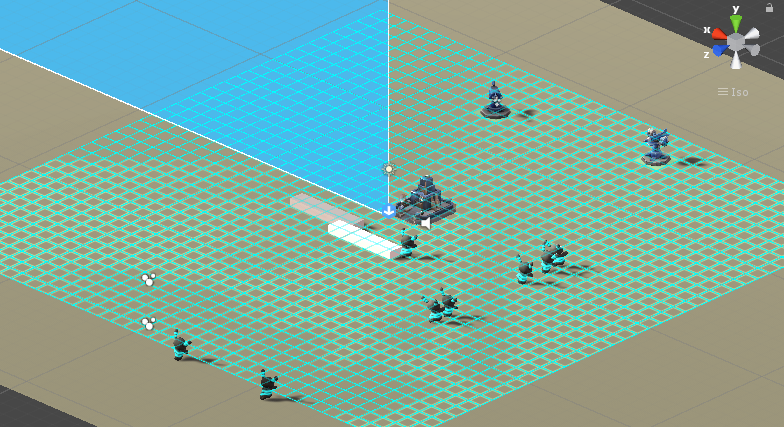
\includegraphics[width=\columnwidth]{InGame2}
	\caption{An in-game image}
\end{figure}

\section{Conclusion}
\begin{itemize}
    \item Synopsis of project
    \item Future work and next steps
\end{itemize}

\section{Acknowledgments}
\begin{itemize}
    \item Use of multiple tutorials/repositories
    \begin{itemize}
        \item Encog Machine Learning Framework
        \item Unity Tower Defense Tutorial
        \item Unity Action Game Shooter Tutorial
        \item Redzen repository for normal random numbers
        \item
    \end{itemize}
\end{itemize}

\footnotesize
\bibliographystyle{apalike}
\bibliography{bibliography} % replace by the name of your .bib file

\end{document}
